\subsection{Layer Operating System}
The front-end, like the entire application, will be run on the browser and will therefore run on any operating system.

\subsection{Layer Software Dependencies}
The entire application will depend on Bootstrap, and the React library.

\subsection{Login Subsystem}
The Login Subsystem will will provide an interface for user to login into the application. Users will be able to login with their email and password credentials or their Google accounts.

\begin{figure}[h!]
	\centering
 	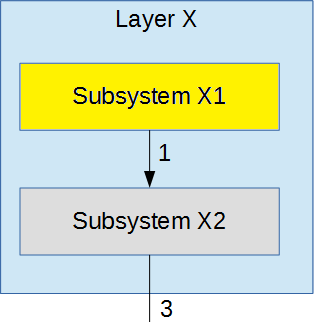
\includegraphics[width=0.60\textwidth]{images/subsystem}
 \caption{Example subsystem description diagram}
\end{figure}

\subsubsection{Subsystem Software Dependencies}
The Login Subsystem will require a consistent connection to the applications database in order to login with their email and password credentials. For a user to login with their Google accounts, the application will depend on the GoogleLogin library.

\subsubsection{Subsystem Programming Languages}
The Login Subsystem will be developed using, React.js, HTML, and CSS.

\subsubsection{Subsystem Data Structures}
A description of any classes or other data structures that are worth discussing for the subsystem. For example, data being transmitted from a microcontroller to a PC via USB should be first be assembled into packets. What is the structure of the packets?

\subsubsection{Subsystem Data Processing}
A description of any algorithms or processing strategies that are worth discussing for the subsystem. If you are implementing a well-known algorithm, list it. If it is something unique to this project, discuss it in greater detail.


